%%%%%%%%%%%%%%%%%%%%%%%%%%%%%%%%%%%%%%%%%%%%%%%%%%%%%%%%%%%%%%%%%%%%%%%%%%%%%%%%
% Template for USENIX papers.
%
% History:
%
% - TEMPLATE for Usenix papers, specifically to meet requirements of
%   USENIX '05. originally a template for producing IEEE-format
%   articles using LaTeX. written by Matthew Ward, CS Department,
%   Worcester Polytechnic Institute. adapted by David Beazley for his
%   excellent SWIG paper in Proceedings, Tcl 96. turned into a
%   smartass generic template by De Clarke, with thanks to both the
%   above pioneers. Use at your own risk. Complaints to /dev/null.
%   Make it two column with no page numbering, default is 10 point.
%
% - Munged by Fred Douglis <douglis@research.att.com> 10/97 to
%   separate the .sty file from the LaTeX source template, so that
%   people can more easily include the .sty file into an existing
%   document. Also changed to more closely follow the style guidelines
%   as represented by the Word sample file.
%
% - Note that since 2010, USENIX does not require endnotes. If you
%   want foot of page notes, don't include the endnotes package in the
%   usepackage command, below.
% - This version uses the latex2e styles, not the very ancient 2.09
%   stuff.
%
% - Updated July 2018: Text block size changed from 6.5" to 7"
%
% - Updated Dec 2018 for ATC'19:
%
%   * Revised text to pass HotCRP's auto-formatting check, with
%     hotcrp.settings.submission_form.body_font_size=10pt, and
%     hotcrp.settings.submission_form.line_height=12pt
%
%   * Switched from \endnote-s to \footnote-s to match Usenix's policy.
%
%   * \section* => \begin{abstract} ... \end{abstract}
%
%   * Make template self-contained in terms of bibtex entires, to allow
%     this file to be compiled. (And changing refs style to 'plain'.)
%
%   * Make template self-contained in terms of figures, to
%     allow this file to be compiled. 
%
%   * Added packages for hyperref, embedding fonts, and improving
%     appearance.
%   
%   * Removed outdated text.
%
%%%%%%%%%%%%%%%%%%%%%%%%%%%%%%%%%%%%%%%%%%%%%%%%%%%%%%%%%%%%%%%%%%%%%%%%%%%%%%%%

%%% Minor updates for SOUPS 2019 by Michelle Mazurek
%%% Minor updates for SOUPS 2022 by Rick Wash

\documentclass[letterpaper,twocolumn,10pt]{article}
\usepackage{usenix2022_SOUPS}

% to be able to draw some self-contained figs
\usepackage{tikz}
\usepackage{amsmath}

% inlined bib file
\usepackage{filecontents}

%-------------------------------------------------------------------------------
\begin{filecontents}{\jobname.bib}
%-------------------------------------------------------------------------------
@Book{arpachiDusseau18:osbook,
  author =       {Arpaci-Dusseau, Remzi H. and Arpaci-Dusseau Andrea C.},
  title =        {Operating Systems: Three Easy Pieces},
  publisher =    {Arpaci-Dusseau Books, LLC},
  year =         2015,
  edition =      {1.00},
  note =         {\url{http://pages.cs.wisc.edu/~remzi/OSTEP/}}
}
@InProceedings{waldspurger02,
  author =       {Waldspurger, Carl A.},
  title =        {Memory resource management in {VMware ESX} server},
  booktitle =    {USENIX Symposium on Operating System Design and
                  Implementation (OSDI)},
  year =         2002,
  pages =        {181--194},
  note =         {\url{https://www.usenix.org/legacy/event/osdi02/tech/waldspurger/waldspurger.pdf}}}
\end{filecontents}

%-------------------------------------------------------------------------------
\begin{document}
%-------------------------------------------------------------------------------

%don't want date printed
\date{}

% make title bold and 14 pt font (Latex default is non-bold, 16 pt)
\title{\Large \bf A Different Kind of Password Manager}

% if you leave this blank it will default to a possibly ugly attempt 
% to make the contents of the \author command below into a string
\def\plainauthor{Author name(s) for PDF metadata. Don't forget to anonymize for submission!}

%for single author (just remove % characters)
\author{
{\rm Alan H.\ Karp}\\
Independent
% copy the following lines to add more authors
% \and
% {\rm Name}\\
%Name Institution
} % end author

\maketitle
\thecopyright

%-------------------------------------------------------------------------------
\begin{abstract}
%-------------------------------------------------------------------------------
Most password managers store passwords so you don't have
to remember them.  That choice imposes costs on the password
manager and risks on its users.  Another option is to calculate
passwords as they are needed.  SitePassword is such a
calculator that provides all the key features that
users want in their password manager -- remembering of metadata, 
synchronization across machines, and autofill capability.
\end{abstract}


%-------------------------------------------------------------------------------
\section{Introduction}\label{intro}
%-------------------------------------------------------------------------------

"Dealing with passwords is awful" is a statement few would disagree
with.  Password managers make the situation less awful, improving both
security and usability.  They make it easier for you to have a different, strong
password for every site while making it convenient to change a password
when necessary.  Of course, users care at least as much about ease of use, trust in the
the password manager, and the ability to get their passwords when 
using a friend's machine as they do the strength of their passwords.

There are two kinds of password managers.  The vast majority of them 
remember passwords and other metadata, such as userids.   They 
make the stored passwords available from any machine by using 
encrypted databases and cloud storage.

Remembering passwords adds cost for the company providing the 
password manager for it to manage user accounts and to pay for the 
necessary cloud storage.  It imposes risks on the user because the
stored passwords can be stolen.

The second kind, password calculators, don't need to store passwords.  They combine a
master password with other data to calculate a strong password
for a website when you need to login.  SitePassword is a
password calculator designed for usability and security that supports all
the features users want.  Usability features are discussed in Section \ref{usability}.

SitePassword remembers your settings for each site and synchronizes them
across your machines without the need for user accounts or cloud storage.
Instead, it puts the metadata in bookmarks, which virtually all browsers
synchronize across machines.  The security aspects of this choice are covered
in Section \ref{security}.  

Using bookmarks makes the settings available on
machines that cannot install the extension, such as mobile devices.  In addition,
there is only a small risk attached to printing the settings, since they only contain
data of limited security value.

%-------------------------------------------------------------------------------
\section{SitePassword Overview}\label{overview}
%-------------------------------------------------------------------------------

SitePassword is an extension that runs in Chromium browsers.\footnote{Brave, 
Chrome, Edge, and Opera.  Firefox is not a pure Chomium Browser.}  
It has three components.  A popup, with the user interface shown in 
Figure \ref{fig:popup}, is where the user provides the necessary metadata.  A
content script is responsible for finding the userid and password fields on the page
and filling them in on request.  A service worker manages the metadata and 
calculates the site password when the content script asks for it.  

\begin{figure}
\begin{center}
  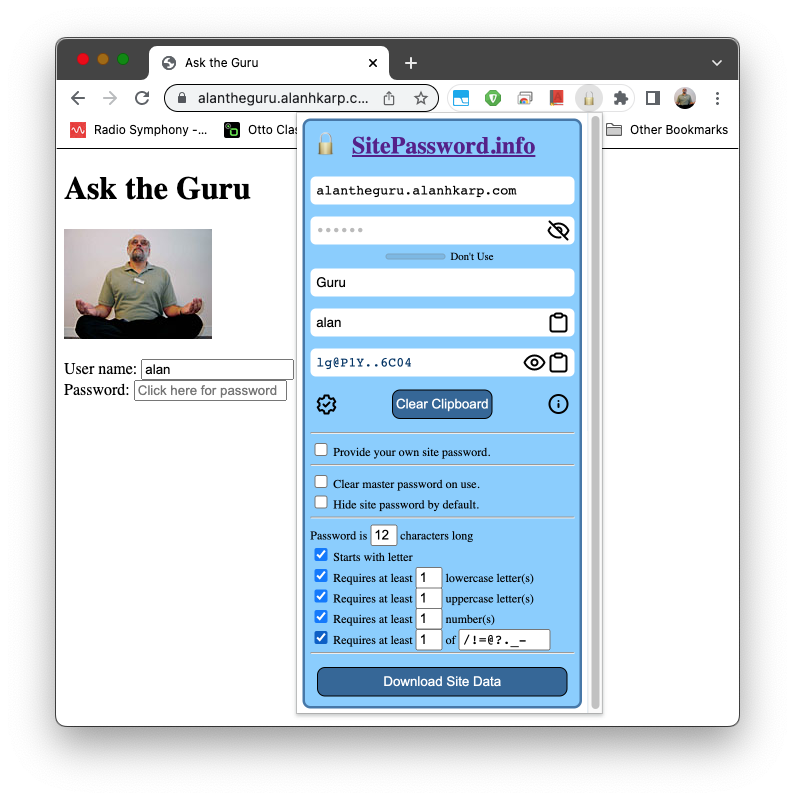
\includegraphics[scale=0.20]{soupsfig1.png}
\end{center}
\caption{\label{fig:popup} The SitePassword popup showing all available
options. }
\end{figure}

When the user first encounters a page with a login form at a given domain, 
the password field contains a placeholder {\em Click SitePassword}.  Clicking
the SitePassword icon opens the popup.  As you fill out the form the site
password field updates on every keystroke, making it clear how uncorrelated
the passwords are.

As you  mouse over to the password field, the userid gets filled in and the placeholder
changes to say {\em Click here for password}.  Click and the password gets
filled in.  When returning to that login page on any machine that synchronizes
your bookmarks and has the extension installed, you only need to click on the 
password field.  The result is that using SitePassword is easier than even typing
the same, weak password for every site.

SitePassword also includes a web page, shown in Figure \ref{fig:webpage}, that can be used to 
get your passwords when the extension is not available, such as on your mobile 
devices.  You don't even have to remember your settings if you synchronize
bookmarks to the device.  You can paste the corresponding bookmark into the form.

\begin{figure}
\begin{center}
  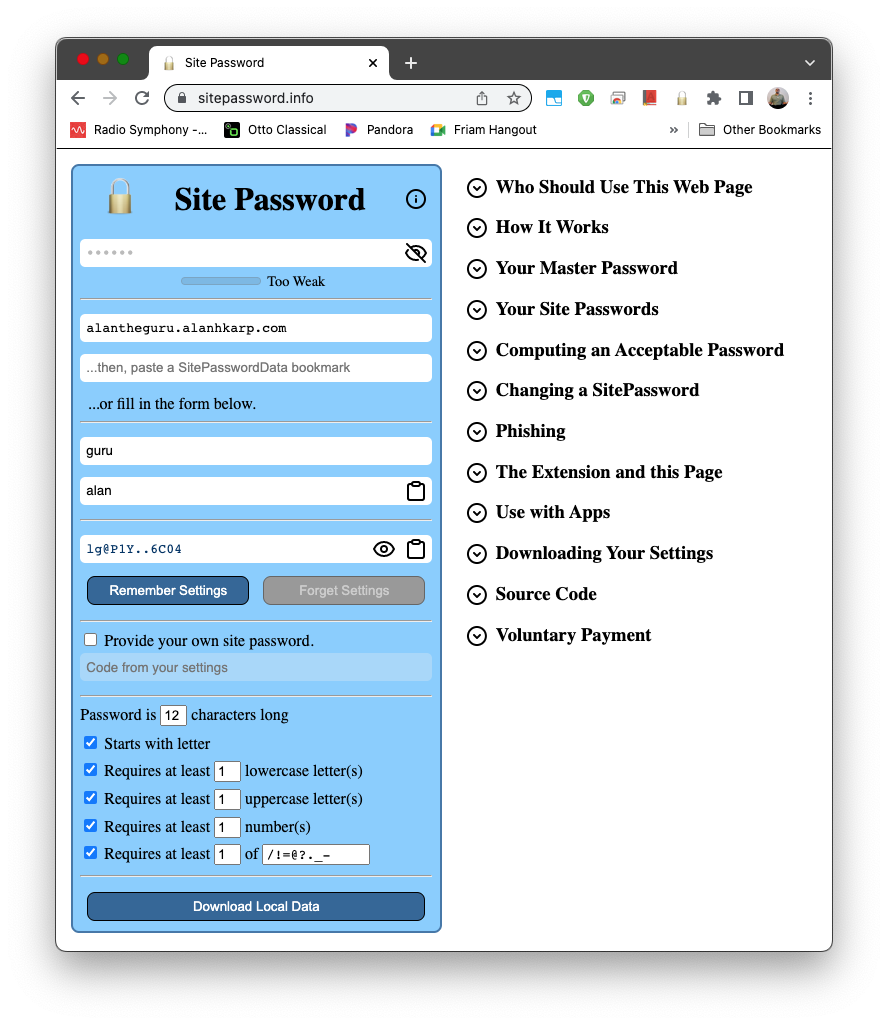
\includegraphics[scale=0.20]{soupsfig2.png}
\end{center}
\caption{\label{fig:webpage} The SitePassword web page showing all available
options and the table of contents of the instructions.  Note that the calculated
password is the same as in Figure 1. }
\end{figure}

Figure \ref{fig:phishing} shows the warning you get if you are at a potential phishing site.  The
detailed message is described in the section on usability.
 
\begin{figure}
\begin{center}
  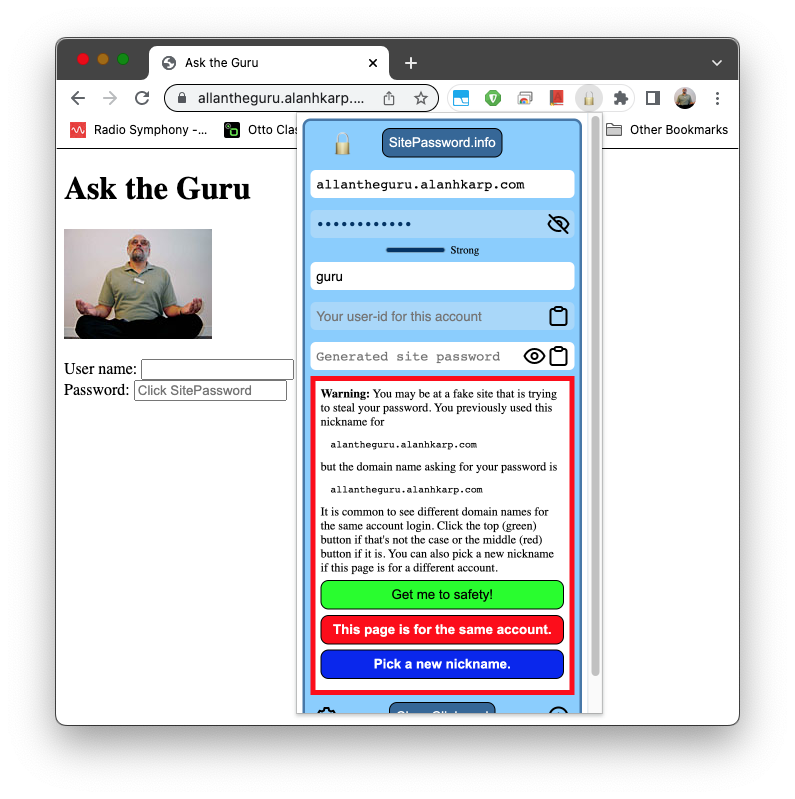
\includegraphics[scale=0.20]{soupsfig3.png}
\end{center}
\caption{\label{fig:phishing} The SitePassword phishing warning. }
\end{figure}

%-------------------------------------------------------------------------------
\section{Usability Considerations}\label{usability}
%-------------------------------------------------------------------------------

People who adopt and then abandon password managers often site usability 
as the main reason.  SitePassword was designed to be as usable as a simple
game.  Each step should be obvious; you should be able to experiment without
worrying about breaking something; warnings make clear what next steps to take.
Although SitePassword comes with extensive instructions, as shown in Figure 2, 
the hope is that they won't be needed.

A very simple way to guide the user is to focus on the field you should fill in next.
Another is to disable fields until they are ready for user interaction.  For example,
the settings that get stored are indexed by the domain name and associated with
the nickname for the site. One choice would be to present an error message to the
user when trying to remember the settings without this information.  Instead, the 
{\em Remember Settings} button is only enabled after that information is available.

Another way to help the user is to provide meaningful labels and tooltips.

%-------------------------------------------------------------------------------
\section{Security Considerations}\label{security}
%-------------------------------------------------------------------------------

%-------------------------------------------------------------------------------
\section{Future Work}\label{improvement}
%-------------------------------------------------------------------------------

%-------------------------------------------------------------------------------
\section{Related Work}\label{related}
%-------------------------------------------------------------------------------

There are a number of reviews of the kind of password manager
that stores passwords, so this section only reviews password calculators.

An early very simple calculator (https://www.hpl.hp.com/techreports/2002/HPL-2002-39R1.html)
hashed the user's master password with a user selected nickname for the site to
produce a password that the user would copy and paste into the password field.  It was 
later adapted into the HP Antiphishing Toolbar for Internet Explorer, which added many
of the features of a modern password manager.

PwdHash (https://www.usenix.org/legacy/events/sec05/tech/full\_papers/ross/ross.pdf) 
combines the user's master password with the domain name of the page.

%-------------------------------------------------------------------------------
\section{Footnotes, Verbatim, and Citations}
%-------------------------------------------------------------------------------

Footnotes should be places after punctuation characters, without any
spaces between said characters and footnotes, like so.%
\footnote{Remember that USENIX format stopped using endnotes and is
  now using regular footnotes.} And some embedded literal code may
look as follows.

\begin{verbatim}
int main(int argc, char *argv[]) 
{
    return 0;
}
\end{verbatim}

Now we're going to cite somebody. Watch for the cite tag. Here it
comes. Arpachi-Dusseau and Arpachi-Dusseau co-authored an excellent OS
book, which is also really funny~\cite{arpachiDusseau18:osbook}, and
Waldspurger got into the SIGOPS hall-of-fame due to his seminal paper
about resource management in the ESX hypervisor~\cite{waldspurger02}.

The tilde character (\~{}) in the tex source means a non-breaking
space. This way, your reference will always be attached to the word
that preceded it, instead of going to the next line.

And the 'cite' package sorts your citations by their numerical order
of the corresponding references at the end of the paper, ridding you
from the need to notice that, e.g, ``Waldspurger'' appears after
``Arpachi-Dusseau'' when sorting references
alphabetically~\cite{waldspurger02,arpachiDusseau18:osbook}. 

It'd be nice and thoughtful of you to include a suitable link in each
and every bibtex entry that you use in your submission, to allow
reviewers (and other readers) to easily get to the cited work, as is
done in all entries found in the References section of this document.

Now we're going take a look at Section~\ref{sec:figs}, but not before
observing that refs to sections and citations and such are colored and
clickable in the PDF because of the packages we've included.

%-------------------------------------------------------------------------------
\section{Floating Figures and Lists}
\label{sec:figs}
%-------------------------------------------------------------------------------

Lists are sometimes quite handy. If you want to itemize things, feel
free:

\begin{description}
  
\item[fread] a function that reads from a \texttt{stream} into the
  array \texttt{ptr} at most \texttt{nobj} objects of size
  \texttt{size}, returning returns the number of objects read.

\item[Fred] a person's name, e.g., there once was a dude named Fred
  who separated usenix.sty from this file to allow for easy
  inclusion.
\end{description}

\noindent
The noindent at the start of this paragraph in its tex version makes
it clear that it's a continuation of the preceding paragraph, as
opposed to a new paragraph in its own right.


\subsection{LaTeX-ing Your TeX File}
%-----------------------------------

People often use \texttt{pdflatex} these days for creating pdf-s from
tex files via the shell. And \texttt{bibtex}, of course. Works for us.

%-------------------------------------------------------------------------------
\section*{Acknowledgments}
%-------------------------------------------------------------------------------

The USENIX latex style is old and very tired, which is why
there's no \textbackslash{}acks command for you to use when
acknowledging. Sorry.


%-------------------------------------------------------------------------------
\bibliographystyle{plain}
\bibliography{\jobname}

%%%%%%%%%%%%%%%%%%%%%%%%%%%%%%%%%%%%%%%%%%%%%%%%%%%%%%%%%%%%%%%%%%%%%%%%%%%%%%%%
\end{document}
%%%%%%%%%%%%%%%%%%%%%%%%%%%%%%%%%%%%%%%%%%%%%%%%%%%%%%%%%%%%%%%%%%%%%%%%%%%%%%%%

%%  LocalWords:  endnotes includegraphics fread ptr nobj noindent
%%  LocalWords:  pdflatex acks
